\section{Il neurone: un sistema del second'ordine}

In questo capitolo studieremo un modello descritto da un'\textbf{equazione differenziale del secondo ordine}, che può essere utilizzato per descrivere vari sistemi che reagiscono a stimoli oltre una certa soglia, ma che può rivelarsi estremamente utile per acquisire nuovi strumenti per l'analisi delle equazioni differenziali più complesse.

\subsection{Comportamenti con soglia} 

Consideriamo un oscillatore armonico sottoposto a smorzamento:
\begin{equation}
	\ddot{x}=-x-\gamma\dot{x} \label{oscillatoreSmorzato}
\end{equation}
vogliamo modificare questa equazione affinchè il comportamento del sistema dipenda fortemente da $x$, nella fattispecie vogliamo modulare lo smorzamento. 

Osserviamo che possiamo modificare il segno del termine di smorzamento per annullarne gli effetti sul sistema. Modifichiamo quindi la (\ref{oscillatoreSmorzato}) con un termine aggiuntivo $1-x^2$ che per $x$ piccolo è positivo ma cambia di segno per $x>1$. Otteniamo quindi: 
\begin{equation}
	\ddot{x}=-x-\gamma(1-x^2)\dot{x} \label{pendoloSoglia}
\end{equation}
questo tipo di sistema è caratterizzato da un comportamento di smorzamento dipendente dalla posizione, per cui oltre un valore soglia, quando $x>1$ il termine di smorzamento cambia segno e il sistema dissipa energia (meccanicamente parlando) e inizia a tendere a $x=0$.

Osserviamo che per $\gamma<0$ si manifesta il comportamento opposto, ossia che oltre un valore soglia il sistema inizia ad assorbire energia e la sua soluzione diverge dalle condizioni iniziali verso infinito.\\

In ogni caso il termine aggiuntivo è in grado, variando il segno di una parte dell'equazione, di introdurre una soglia oltre la quale il comportamento del sistema muta. 

\subsection{Riduzione al prim'ordine}

Il termine moltiplicativo che abbiamo aggiunto ha però lo svantaggio di rendere più complessa la risoluzione dell'equazione differenziale (\ref{pendoloSoglia}).\\

Introduciamo una nuova variabile per poter ridurre l'ordine dell'equazione differenziale aumentandone la dimensione:
\begin{equation*}
	\dot{y}=-\frac{x}{\gamma} \Rightarrow  \ddot{x}=\gamma \dot{y}-\gamma(1-x^2)\dot{x} 
\end{equation*}

Integrando otteniamo il sistema:
\begin{equation}
	\begin{cases}
		\dot{x}=\gamma y+\gamma(x-\frac{x^3}{3})\\
		\dot{y}=-\frac{x}{\gamma}
		\label{sistema}
	\end{cases}
\end{equation}

Dobbiamo quindi studiare il sistema (\ref{sistema}) per poter comprendere meglio le proprietà del modello. Come già fatto per l'equazione logistica iniziamo studiando i punti di equilibrio, ossia quando $\dot{x}=0$ e $\dot{y}=0$; ogni singola condizione definisce in una sorta di spazio delle fasi $(x,y)$ i luoghi dei punti in cui il sistema è in equilibrio rispetto ad $x$ o $y$, queste curve sono dette \textbf{nullcline}, dall'inglese \emph{nullclines}, e risulteranno fondamentali per comprendere qualitativamente l'evoluzione del sistema.
\begin{multicols}{2}
	\begin{center}
	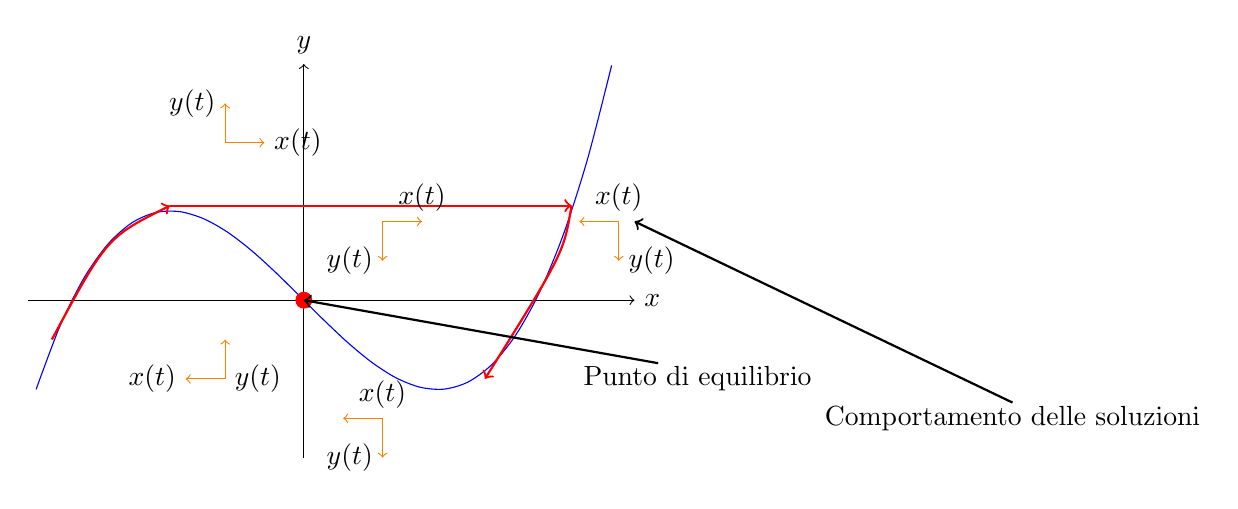
\begin{tikzpicture}
			\draw[->] (-3.5, 0) -- (4.2, 0) node[right] {$x$};
			\draw[->] (0, -2) -- (0, 3) node[above] {$y$};
			\draw[scale=1.7, domain=-2:2.3, smooth, variable=\x, blue] plot ({\x}, {-\x+\x*\x*\x/3});
			
			\draw[draw=red, thick, ->] (-3.2,-0.5) .. controls (-2.5,0.8) .. (-1.7,1.2);
			\draw[draw=red, thick, ->] (-1.7,1.2) -- (3.4,1.2);
			\draw[draw=red, thick, ->] (3.4,1.2) .. controls (3.3,0.6) .. (2.3,-1);
			
			\draw[draw=orange,->] (1,1) -- (1.5,1) node[above] {$x(t)$};
			\draw[draw=orange,->] (1,1) -- (1,0.5) node[left] {$y(t)$};
			\draw[draw=orange,<-] (3.5,1) -- (4,1) node[above] {$x(t)$};
			\draw[draw=orange,->] (4,1) -- (4,0.5) node[right] {$y(t)$};
			\draw[draw=orange,<-] (0.5,-1.5) -- (1,-1.5) node[above] {$x(t)$};
			\draw[draw=orange,->] (1,-1.5) -- (1,-2) node[left] {$y(t)$};
			\draw[draw=orange,->] (-1,-1) -- (-1.5,-1) node[left] {$x(t)$};
			\draw[draw=orange,<-] (-1,-0.5) -- (-1,-1) node[right] {$y(t)$};
			\draw[draw=orange,->] (-1,2) -- (-0.5,2) node[right] {$x(t)$};
			\draw[draw=orange,->] (-1,2) -- (-1,2.5) node[left] {$y(t)$};
			
			\filldraw[draw=red,fill=red] (0,0) circle (0.1cm);
			\draw[thick, <-] (0,0) -- (4.5,-0.8);
			\node[] at (5,-1) {Punto di equilibrio};
			\draw[thick, <-] (4.2,1) -- (9,-1.3);
			\node[] at (9,-1.5) {Comportamento delle soluzioni};
			
	\end{tikzpicture}
\end{center}
\begin{align*}
	Nullcline\quad\Rightarrow\quad
	\begin{cases}
			x=0\\
		y=\frac{x^3}{3}-x
	\end{cases}\\
	\begin{cases}
		x>0\quad \Rightarrow \quad \dot{y}<0\\
		y>\frac{x^3}{3}-x \quad \Rightarrow \quad \dot{x}>0
	\end{cases}
\end{align*}

\end{multicols}	

Osserviamo subito che il punto di equilibrio complessivo del sistema è dato dall'intersezione delle nullcline, poiché in questi punti sia $\dot{x}$ e $\dot{y}$ si annullano: nel nostro caso questo avviene nell'origine.\\

In secondo luogo osserviamo che le nullcline separano il piano in due regioni ciascuna, ognuna dove la variabile della nullclina cresce o decresce, infatti annullandosi $\dot{x}$ e $\dot{y}$ sulle curve abbiamo che queste delimitano le regioni dove $\dot{x}$ e $\dot{y}$ hanno segni diversi e quindi dove varia la monotonia della soluzione.\\

Definiamo ora \textbf{variabile veloce} la variabile che cresce più rapidamente nella dinamica del sistema e conseguentemente definiamo la \textbf{variabile lenta}.\\ In questo caso è semplice distinguerle infatti sappiamo che $\dot{y}=-\frac{x}{\gamma}$, il che per $\gamma$ grandi rende molto più lenta la crescita di $y$ rispetto a quella di $x$, che infatti è la variabile veloce. Per lo studio del sistema riconoscere queste differenze è fondamentale infatti il sistema cercherà di evolvere seguendo la dinamica della variabile veloce e, ove è possibile, la sua nullclina. \\

Infine osserviamo che il moto sulla nullclina veloce non sempre è compatibile con la dinamica locale del sistema: immaginiamo di portare il sistema a $x$ e $y$ negativi sulla nullclina di $\dot{x}$, in questo caso $\dot{x}=0$, per cui verrà seguita la dinamica di $y$ sulla nullcina stessa, infatti abbiamo già detto che per $x<0$ si ha che $\dot{y}>0$ per cui il sistema tenderà a risalire verso l'origine del piano. \\
Giunto al primo massimo locale il sistema, per seguire la nullclina, dovrebbe far decrescere $y$, cosa non concessa dalla condizione $\dot{y}>0$. In questo caso è la dinamica veloce di $x$ a spostare il sistema dal punto di massimo alla regione con $x>0$ mantenendo $y$ circa costante, in tempi molto brevi, fino ad incontrare nuovamente la nullclina in un punto dove il moto sulla curva sarà di nuovo concorde con le condizioni locali sulle derivate prime.\\

Questo tipo di comportamento genera un'orbita stabile attorno all'origine che però è un punto di equilibrio instabile poichè è situato in una zona \textbf{proibita} delle nullcline.\\ Se però $\gamma$ fosse stato negativo l'origine sarebbe chiaramente stata un punto stabile, come già osservato all'inizio. Questo tipo di fenomeno attorno ai punti di equilibrio prende il nome di \textbf{Biforcazione di Hopf}. 

\subsection{Il modello del neurone}

Quanto abbiamo appena compreso si rivela utile per la comprensione del modello matematico utilizzato per descrivere la risposta ad impulsi elettrici dei neuroni. Chiamiamo $x$ la tensione nel neurone, $w$ la corrente che vi scorre all'interno e $I$ un ipotetico stimolo esterno che il neurone può ricevere, allora:
\begin{equation}
		\dot{x}=x-\frac{x^3}{3}-w+I \qquad
		\dot{w}=\frac{x+a-bw}{\gamma}
\end{equation} 
Come già abbiamo fatto procediamo a studiare le nullcline, i punti di equilibrio e le variabili del sistema. Chiaramente è $x$ la variabile veloce.
\begin{multicols}{2}
	\begin{center}
		\begin{tikzpicture}
			\draw[->] (-3.5, 0) -- (2.7, 0) node[right] {$x$};
			\draw[->] (0, -2) -- (0, 2) node[above] {$w$};
			\draw[scale=1.7, domain=-2:1.5, smooth, variable=\x, blue] plot ({\x}, {+\x-\x*\x*\x/3-0.5});
			\draw[scale=1.7, domain=-2:1.3, smooth, variable=\x, blue] plot ({\x}, {\x+0.5});
			
			
		\end{tikzpicture}
	\end{center}

    Lo studio delle nullcline evidenzia che esiste un punto di equilibrio, infatti non è possibile costruire le due curve senza che si intersechino, non sappiamo però nulla sulla sua stabilità. \\
    
    Procediamo quindi a studiare le perturbazioni vicino all'equilibrio linearizzando il sistema di equazioni differenziali.
\end{multicols}
\begin{multicols}{2}
\begin{align*}
	\delta x=x-x_{eq} \qquad \qquad \quad \delta w=w-w_{eq}\\
	\delta \dot{x}=(1-x^2_{eq})\delta x-\delta w \qquad \delta \dot{w}=\frac{\delta x -b\ \delta w}{\gamma}
\end{align*}
\begin{align*}
	\\\\
	\begin{pmatrix}
		\dot{x} \\
		\dot{w}
	\end{pmatrix}
	=
	\begin{pmatrix}
		1-x_{eq}^2 & -1 \\
		\frac{1}{\gamma} & -\frac{b}{\gamma}
	\end{pmatrix}
	\begin{pmatrix}
		x \\
		w
	\end{pmatrix}
=
M\begin{pmatrix}
	x \\
	w
\end{pmatrix}
\end{align*}
\end{multicols}
Ora possiamo studiare la traccia e il determinante della matrice che caratterizza il sistema linearizzato per capire quali condizioni rendono entrambi gli autovalori negativi così che le perturbazioni convergano verso il punto di equilibrio.

\begin{align}
\det(M)= -\frac{b}{\gamma}(1-x^2_{eq})+\frac{1}{\gamma}\propto\lambda_1\ \lambda_2\\
Tr (M)=(1-x^2_{eq})-\frac{b}{\gamma}\propto\lambda_1+\lambda_2
\end{align}

Risulta chiaro che per $x_{eq}^2>>0$ gli autovalori sono negativi per cui l'equilibrio è stabile e viceversa per $x_{eq}^2$ che tende a zero.\\

Infine osserviamo che il termine $I$ costituisce un paramento di traslazione verticale per la nullclina di $\dot{x}$, questo quindi regola a che distanza dell'origine è collocato il punto di equilibrio e quindi la sua stabilità. Possiamo però anche vedere questo termine come dipendente dal tempo e nella fattispecie nella forma $\Delta I\ \delta(t)$, ossia del prodotto tra un termine costante e una Delta di Dirac. Così facendo l'integrazione di questo termine ha l'effetto di cambiare le condizioni iniziali del sistema che si troverà lontano dal punto di equilibrio.

A questo punto se $\Delta I$ è grande a sufficienza e il punto di equilibrio è stabile  il sistema inizierà ad orbitare attorno al punto di equilibrio come avviene per il biforcamento di Hopf, ossia separandosi dalla nullclina, in maniera tale da generare una crescita rapida che va poi a decadere nel tempo come risposta allo stimolo esterno. Se $\Delta I$ invece non è sufficientemente grande il sistema oscillerà attorno all'equilibrio senza generare un risposta.
\begin{center}
	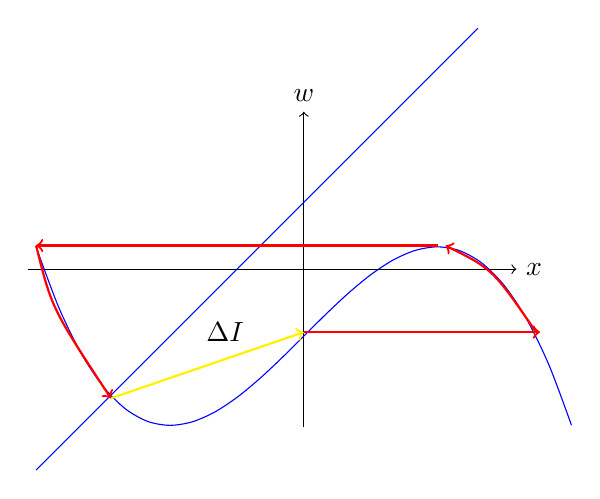
\begin{tikzpicture}
		\draw[->] (-3.5, 0) -- (2.7, 0) node[right] {$x$};
		\draw[->] (0, -2) -- (0, 2) node[above] {$w$};
		\draw[scale=1.7, domain=-2:2, smooth, variable=\x, blue] plot ({\x}, {+\x-\x*\x*\x/3-0.5});
		\draw[scale=1.7, domain=-2:1.3, smooth, variable=\x, blue] plot ({\x}, {\x+0.5});
		
		\draw[thick ,draw=yellow, ->] (-2.45,-1.64) -- (0,-0.8);
		\draw[thick, draw=red, ->] (0,-0.8) -- (3,-0.8) ;
		\draw[thick, draw=red, ->] (2.95,-0.8) .. controls (2.4,0) ..(1.8,0.3);
		\draw[thick, draw=red, ->] (1.7,0.3) -- (-3.4,0.3) ;
		\draw[thick, draw=red, ->] (-3.4,0.3) .. controls (-3.2,-0.5) ..(-2.45,-1.64);
		\node at (-1,-0.8) {$\Delta I$};
		
	\end{tikzpicture}
\end{center}

Abbiamo quindi ottenuto un sistema in grado di rispondere a stimoli esterni con un meccanismo di soglia che nei neuroni è utilizzato per evitare scariche anomale nel sistema nervoso, cosa che per esempio non viene evitata durante un attacco epilettico.

